% !TEX root = chapter-standalone.tex


\chaptersecond{Monotone Design Theory}{chapter-swissarmyknife}{}{


    This chapter introduces  \emph{Monotone Design Theory}, a formalization for computational design theory.
    It is a compositional theory of which the primitive elements are \emph{design problems} (DPI),
    formalized as a relations among functionality, resources, and implementations.

    We show that DPIs can capture design problems across diverse fields.

}
\todotextjira{297}{We start right away talking about monotonicity after the DPI definition, but the link is not clear.}


\label{ch:design-problems}
% !TEX root = chapter-standalone.tex


\section{Design Problems}
\label{sec:Design-Problems}

We start by defining a ``design problem with implementation'', which is a tuple of ``\F{functionality} space'',
``\Icol{implementation} space'', and ``\R{resources} space'', together with two maps that describe the feasibility relations between these three spaces (\cref{fig:setup}).

\begin{definition}[Design problem with implementation]
  \label{def:DPI}
  A \emph{\iindex{design problem with implementation}} (DPI) is a tuple
  \begin{equation}
    \tup{\funsp, \ressp, \impsp, \prov,\req},
  \end{equation}
  where:

  \begin{compactitem}
    \item \funsp is a poset, called \emph{\Fcol{functionality} space};
    \item \ressp is a poset, called \emph{\Rcol{requirements} space};
    \item \impsp is a set, called \emph{\Icol{implementation} space};
    \item the map~$\prov\colon\impsp\rightarrow\funsp$
    maps an implementation to the functionality it provides;
    \item the map~$\req\colon\impsp\rightarrow\ressp$
    maps an implementation to the resources it requires.
  \end{compactitem}

\end{definition}

\begin{figure}[h]
  \begin{center}
    \includesag{funimpres_1}
  \end{center}
  \caption{\label{fig:setup}}
\end{figure}

\devel{
\begin{forslides}
  \begin{equation*}
\label{eq:fun_poset}
\tup{\funsp, \preceq_{\funsp}}
\end{equation*}
\begin{equation*}
\label{eq:res_poset}
\tup{\ressp, \preceq_{\ressp}}
\end{equation*}
  \begin{equation*}
    \label{eq:decl_dp}
    \adp \colon \funsp \profto \ressp
\end{equation*}
    \begin{equation*}
    \label{eq:decl_dp_1}
    \adpa \colon \funspa \profto \resspb
\end{equation*}
      \begin{equation*}
    \label{eq:decl_dp_std}
    \adp \colon \funsp \op \times \ressp \toinPos \Bool
\end{equation*}
      \begin{equation*}
    \label{eq:decl_dp_2}
    \adpb \colon \funspb \profto \resspc
\end{equation*}
        \begin{equation*}
    \label{eq:decl_dp_3}
    (\adpa\fthen \adpb) \colon \funspa \profto \resspc
\end{equation*}
  \begin{equation*}
    \label{eq:opt_1}
    \res_k\in \tup{\ressp_k,\posleq_{\ressp_k}}
\end{equation*}
    \begin{equation*}
    \label{eq:opt_2}
    \fun_k\in \tup{\funsp_k,\posleq_{\funsp_k}}
\end{equation*}
    \begin{equation*}
    \label{eq:opt_3}
    \adp_k\colon \funsp_k\op \profto \ressp_k
\end{equation*}
    \begin{equation*}
    \label{eq:opt_4}
    \adp_k(\fun_k^*,\res_k)=\true
\end{equation*}
      \begin{equation*}
    \label{eq:opt_5}
    \res_i\posleq \fun_j
\end{equation*}
        \begin{equation*}
    \label{eq:opt_6}
    \Min_{\posleq}\bar{\res}
\end{equation*}
  \begin{equation*}
    \label{eq:genfun_1}
    \ressp
\end{equation*}
    \begin{equation*}
    \label{eq:genfun_2}
    \funsp
\end{equation*}
    \begin{equation*}
    \label{eq:genfun_3}
    \ressp_1
\end{equation*}
      \begin{equation*}
    \label{eq:genfun_3_1}
    \ressp_2
\end{equation*}
        \begin{equation*}
    \label{eq:genfun_3_2}
    \ressp_1\times \ressp_2
\end{equation*}
    \begin{equation*}
    \label{eq:genfun_4}
    \funsp_1
\end{equation*}
    \begin{equation*}
    \label{eq:genfun_5}
    \funsp_2
\end{equation*}
      \begin{equation*}
    \label{eq:genfun_6}
    \fun_1
\end{equation*}
        \begin{equation*}
    \label{eq:genfun_7}
    \fun_2
\end{equation*}
          \begin{equation*}
    \label{eq:genfun_8}
    \res
\end{equation*}
\begin{equation*}
    \label{eq:genfun_9}
    \begin{aligned}
      \ftor_\mathrm{loop}\colon \funsp_1 &\mto \antichains(\ressp)\\
      \fun_1&\mapsto \text{least-fixed-point}(\Phi_{\fun_1})
  \end{aligned}
\end{equation*}
  \begin{equation*}
    \label{eq:genfun_10}
    \begin{aligned}
      \Phi_{\fun_1}\colon \antichains(\ressp)&\mto \antichains(\ressp)\\
      \R{S}&\mapsto \Min_{\posleq_\ressp} \bigcup_{\res \in \R{S}}\ftor(\fun_1,\res)\cap \upit \res
  \end{aligned}
\end{equation*}
            \begin{equation*}
    \label{eq:genfun_11}
    \R{S}\subset \antichains(\ressp)
\end{equation*}
              \begin{equation*}
    \label{eq:genfun_12}
    \R{S_0}=\{ \bot_\ressp\}
\end{equation*}
\begin{equation*}
    \label{eq:genfun_13}
    \R{S_{k+1}}=\Phi_{\fun_1}(\R{S_k})
\end{equation*}
  \begin{equation*}
    \label{eq:genfun_14}
    \bot_{\ressp}
\end{equation*}
\includesag{520_battery}
  \includesag{520_particle_filters}
\includesag{520_chassis_comp}
  \includesag{520_motor_comp}
  \includesag{520_motor_chassis_comp}
  \includesag{520_imp_comp}
\includesag{generic_dp_1}
  \includesag{generic_dp_2}
  \includesag{generic_dp_comp}
  \includesag{edge_opt_dp}
  \includesag{node_opt_dp}
  \includesag{generic_dp_3}
  \includesag{generic_dp_4}
  \includesag{bin_packing_dp}
\begin{equation*}
  \label{eq:imp_comp}
  \impsp \subseteq \impsp_{1} \setconcat \impsp_{2}
\end{equation*}
\end{forslides}
}


A graphical notation will help reasoning about composition. A DPI is represented as a box with~$\dpinumf$ green edges and~$\dpinumr$ red edges~(\cref{fig:dp_graphical}).

\begin{figure}[h]
  \centering
  \includesag{520_general_dp}
  \caption{\label{fig:dp_graphical}}
\end{figure}

%\captionsideleft{\label{fig:dp_graphical}}{\includegraphics[scale=0.33]{gmcdp_dp_graphical.pdf}}

This means that the functionality and resources spaces can be factorized in~$\dpinumf$ and~$\dpinumr$ components:
\begin{equation*}
  \funsp=\prod_{i=1}^{\dpinumf}\pi_{i}\funsp_{i},\quad \ressp=\prod_{j=1}^{\dpinumr}\pi_{j}\ressp_{j},
\end{equation*}
where ``$\pi_{i}$'' represents the projection to the~$i$-th component.
If there are no \textF{green} (respectively, \textR{red}) edges, then~$\dpinumf$ (respectively,~$\dpinumr$) is zero, and \funsp (respectively, \ressp) is equal to~$\One=\{\emptytuple \}$, the set containing one element, the empty tuple~$\emptytuple$.
\todotext{The $\One$ used above might clash with other parts}

These \emph{co-design diagrams} are not to be confused with signal flow diagrams, in which the boxes represent oriented systems and the edges represent signals.


\begin{example}
  \label{exa:dpi_elmotor}
  We now want to revisit the leading example of \cref{sec:attributes_sameness} with the newly introduced co-design perspective. Let's consider a list of electrical motors as in~\cref{tab:electric_motors_2}.
  \begin{table*}[h]
    \centering
    \adjustbox{max width=\textwidth}{%
      \begin{tabular}{c|c|c|c|c|c}
        Motor ID & Company & $\unit[\text{Torque}]{[kg\cdot cm]}$ & \unit[Weight]{[g]} & \unit[Max Power]{[W]}
        & \unit[Cost]{[USD]}
        \\
        \hline
        \textsf{1204} & \textsf{SOYO}        & 0.18 & 60.0  & 2.34 & 19.95  \\
        \textsf{1206} & \textsf{SOYO}        & 0.95 & 140.0 & 3.00 & 19.95  \\
        \textsf{1207} & \textsf{SOYO}        & 0.65 & 130.0 & 2.07 & 12.95  \\
        \textsf{2267} & \textsf{SOYO}        & 3.7  & 285.0 & 4.76 & 16.95  \\
        \textsf{2279} & \textsf{Sanyo Denki} & 1.9  & 165.0 & 5.40 & 164.95 \\
        \textsf{1478} & \textsf{SOYO}        & 19.0 & 1,000 & 8.96 & 49.95  \\
        \textsf{2299} & \textsf{Sanyo Denki} & 2.2  & 150.0 & 5.90 & 59.95
      \end{tabular}%
    }
    \caption{A simplified catalogue of motors.}
    \label{tab:electric_motors_2}
  \end{table*}

  We can think of this as a catalogue of electric motors~$\tup{\impsp_\mathrm{EM},\prov_\mathrm{EM},\req_\mathrm{EM}}$.
  In particular, the set of implementations collects all the motor models, which we can specify using the motor IDs:
  \begin{equation}
    \impsp_\mathrm{EM}=\{1204,1206,1207,2267,2279,1478,2299 \}.
  \end{equation}
  We now have to think about \textR{resources} and \textF{functionalities}.
  Each motor \textR{requires} some \textR{weight} (in \unit[]{g}), \textR{power} (in \unit[]{W}), and has some \textR{cost} (in USD), and \textF{provides} some \textF{torque} (in~$\unit[]{kg\cdot cm}$).
  Thus, we can identify
  \begin{equation*}
    \funsp =\reals\times \{\unit[]{kg\cdot cm}\},\quad \ressp=(\reals\times \{\unit[]{g}\})\times (\reals\times \{\unit[]{W}\})\times (\reals\times \{\unit[]{USD}\}),
  \end{equation*}
  by considering the units as discussed in \cref{sec:currency_cat}.
  The correspondences are given by the details in \cref{tab:electric_motors_2}.
  For instance, we have
  \begin{equation}
    \prov_\mathrm{EM}(1204)=\unit[0.18]{kg\cdot cm}, \quad \req_\mathrm{EM}(1204)=\tup{\unit[60]{g},\unit[2.34]{W},\unit[19.95]{USD}}.
  \end{equation}

  \begin{comment}

  \begin{table}[tbh]
    \begin{center}
      \begin{tabular}{cccc}
        Technology & Specific energy [\unitfrac[]{J}{kg}] & Specific cost [\unitfrac[]{J}{\stdcurr}]
        & Life [\# cycles]
        \\
        \hline
        $\mathsf{NiMH}$  & 100.0 & 3.41 & 500    \\
        $\mathsf{NiH2}$  & 45.0  & 10.5 & 20,000 \\
        $\mathsf{LCO}$   & 195.0 & 2.84 & 750    \\
        $\mathsf{LMO}$   & 150.0 & 2.84 & 500    \\
        $\mathsf{NiCad}$ & 30.0  & 7.50 & 500    \\
        $\mathsf{SLA}$   & 30.0  & 7.00 & 500    \\
        $\mathsf{LiPo}$  & 250.0 & 2.50 & 600    \\
        $\mathsf{LFP}$   & 90.0  & 1.50 & 1,500
      \end{tabular}
    \end{center}
    \caption{Specifications of common battery technologies~\cite{censi2015}. }
    \label{tab:battery}
  \end{table}
\end{comment}

\end{example}


\begin{example}[Motor design]
  \label{exa:motor}
  Suppose we need to choose a motor for a robot from
  a given set. The \emph{functionality} of a motor could be parametrized
  by \textF{torque} and \textF{speed}. The \emph{resources} to consider
  could include the \R{\unit[cost]{[USD]}}, the \R{\unit[mass]{[g]}}, the
  input \R{\unit[voltage]{[V]}}, and the input \R{\unit[current]{[A]}}.
  The map~$\prov \colon \impsp\to\funsp$ assigns to each motor its
  functionality, and the map~$\req \colon \impsp\rightarrow\ressp$ assigns
  to each motor the resources it needs~(\cref{fig:motor_evalexec}).
\end{example}

\begin{figure}[h]
  \centering
  %\includegraphics[scale=0.4]{gmcdp_motor_evalexec}
  \includesag{motor_evalexec}
  \caption{}
  \label{fig:motor_evalexec}
\end{figure}
%\captionsideleft{\label{fig:motor_evalexec}}{\includegraphics[scale=0.33]{gmcdp_motor_evalexec}}

\begin{example}[Chassis design]
  \label{exa:chassis}
  Suppose we need to choose a chassis for a robot~(\cref{fig:gmcdp_chassis_eval}).
  The implementation space~\impsp could be the set of all chassis that could ever be designed (in case of a theoretical analysis),
or just the set of chassis available in the catalogue at hand (in case of a practical design decision).
  The functionality of a chassis could be formalized as ``the ability to transport a certain \F{payload
      {[}g{]}}'' and ``at a given \F{speed {[}m/s{]}}''.
  More refined functional requirements would include maneuverability, the cargo volume, \etc.
  The resources to consider could be the \R{cost {[}USD{]}} of the chassis; the total mass;
and, for each motor to be placed in the chassis, the required \R{speed {[}rad/s{]}} and \R{torque {[}Nm{]}}.
\end{example}

\begin{figure}[h]
  \centering
  \includesag{chassis_execeval}
  \caption{}
  \label{fig:gmcdp_chassis_eval}
\end{figure}


%\begin{forslides}
\devel{
\begin{center}
\includesag{funresuplow_1}
\end{center}
}
%\end{forslides}

%\captionsideleft{\label{fig:gmcdp_chassis_eval}}{\includegraphics[scale=0.33]{gmcdp_chassis_eval.pdf}}

\subsection{Mechatronics}
Many mechanisms can be readily modeled as relations between a provided  functionality and required resources.

\begin{example}
  The \textF{functionality} of a DC motor~(\cref{fig:dc_motor}) is to provide a certain \textF{speed} and \textF{torque}, and the \textR{resources} are \textR{current} and \textR{voltage}.
\end{example}

\begin{figure}[h]
  \begin{center}
    \includesag{520_dc_motor}
  \end{center}
  \caption{\label{fig:dc_motor}}
\end{figure}


\begin{example}
  A gearbox (\cref{fig:gearbox}) provides a certain \textF{output
  torque~$\tau_o$} and \textF{speed~$\tau_o$}, given a certain
  \R{input torque $\tau_i$} and \R{speed $\omega_i$}. For
  an ideal gearbox with a reduction ratio $r \in \ratnumbers_+$ and
  efficiency ratio $\gamma$, $0<\gamma<1$, the constraints among
  those quantities are ${\colR \omega_i}\geq r\,{\colF \omega_o}$
  and ${\colR \tau_i\omega_i}\geq\gamma\,{\colF \tau_o\omega_o}.$
\end{example}

\begin{figure}[h]
  \begin{center}
    \includesag{520_dp_gearbox}
  \end{center}
  \caption{}
  \label{fig:gearbox}
\end{figure}


\begin{example}
  \emph{Propellers}~(\cref{fig:propeller}) generate \F{thrust}
  given a certain \R{torque} and \R{speed}.
\end{example}

\begin{figure}[h]
  \begin{center}
    \includesag{520_dp_propellers}
  \end{center}
  \caption{\label{fig:propeller}}
\end{figure}

\begin{example}
  A \emph{crank-rocker} (\cref{fig:crack}) converts \R{rotational
  motion} into a \F{rocking motion}.
\end{example}

\begin{figure}[h]
  \centering
  \includesag{520_crank}
  \caption{\label{fig:crack}}
\end{figure}

\subsection{Geometrical constraints}

Geometrical constraints are examples of constraints that are easily recognized as monotone, but possibly hard to write down in closed form.

\begin{example}[Bin packing]
  Suppose that each internal component occupies a volume
  bounded by a parallelepiped, and that we must choose the minimal enclosure
  in which to place all components~(\cref{fig:packing}). What
  is the minimal size of the enclosure? This is a variation of the \emph{bin
  packing} problem, which is in NP for both 2D and 3D~\cite{lodi02two}.
  It is easy to see that the problem is monotone, by noticing that,
  if one the components shapes increases, then the size of the enclosure
  cannot shrink.
\end{example}

\begin{figure}[h]
  \centering
  
\includegraphics[scale=0.33]{reits2_fit_boxes}
  \caption{\label{fig:packing}}
\end{figure}
\todographics{Add pics as res/fun}

\subsection{Inference}

Many inference problems have a monotone formalization, taking the
\F{accuracy} or \F{robustness} as functionality, and \R{computation}
or \R{sensing} as resources. Typically these bounds are known in
a closed form only for restricted classes of systems, such as the
linear/Gaussian setting.

\begin{example}
(SLAM)
  One issue with particle-filter-based estimation procedures,
  such as the ones used in the popular GMapping~\cite{grisetti07improved}
  method, is that the filter might diverge if there aren't enough particles.
  Although the relation might be hard to characterize, there is a monotone
  relation between the \F{robustness} (1 - probability of failure),
  the \F{accuracy}, and the \R{number of particles}~(\cref{fig:gmapping}).
\end{example}

\begin{figure}[h]
  \centering
  \includesag{520_mapping}
  \caption{\label{fig:gmapping} }
\end{figure}



\begin{example}
(Stereo reconstruction)
  Progressive reconstruction systems (\cite{locher16progressive}),
  which start with a coarse approximation of the solution that is progressively
  refined, are described by a smooth relation between the \F{resolution}
  and the \R{latency} to obtain the answer~(\cref{fig:progressive}).
  A similar relation characterizes any anytime algorithms in other domains,
  such as robot motion planning.
\end{example}


\begin{figure}[h]
  \centering
  \includesag{520_stereo}
  \caption{\label{fig:progressive}}
\end{figure}


\begin{example}
  The empirical characterization of the monotone relation between \F{the
  accuracy of a visual SLAM solution} and \R{the power consumption}
  is the goal of recent work by Davison and colleagues~\cite{nardi15introducing,zia16comparative}.
\end{example}

\todographics{Reproduce plot from paper.}

\subsection{Communication}

\begin{example}[Transducers]
  Any type of "transducer" that bridges between different
  mediums can be modeled as a DP. For example, an access point~(\cref{fig:accesspoint})
  provides the \F{"wireless access"} functionality, and requires
  that the infrastructure provides the \R{"Ethernet access"} resource.
\end{example}


\begin{figure}[h]
  \centering
  \includesag{520_ethernet}
  \caption{\label{fig:accesspoint}}
\end{figure}

\begin{example}[Wireless link]
  The basic functionality of a wireless link is to provide
  a certain \F{bandwidth} (\cref{fig:networklink}). Further refinements could include bounds
  on the latency or the probability that a packet drop is dropped. Given
  the established convention about the the preference relations for
  functionality, in which a \emph{lower} functionality is "easier"
  to achieve, one needs to choose "\F{\emph{minus} the latency}"
  and "\F{\emph{minus} the packet drop probability}" for them
  to count as functionality. As for the resources, apart from the \R{transmission
  power [W]}, one should consider at least \R{the spectrum occupation},
  which could be described as an interval~$[f_0,f_1]$ of the frequency
  axis $\reals^{\unit[]{[Hz]}}$. Thus the resources space is $\ressp=\colR\reals^{\unit[]{[W]}}\times\aword{intervals}(\reals^{\unit[]{[Hz]}})$.
\end{example}

\begin{figure}[h]
  \begin{center}
    \includesag{520_dp_wireless}
  \end{center}
  \caption{ \label{fig:networklink}}
\end{figure}

\subsection{Multi-robot systems}

In a multi-robot system there is always a trade-off between the number
of robots and the capabilities of the single robot.
\begin{example}
  Suppose we need to create a swarm of agents whose functionality is
  \F{to sweep an area}. If the functionality is fixed, one expects
  a three-way trade-off between the three resources: number of agents,
  the speed of a single agent, and the execution time. For example,
  if the time available decreases, one has to increase either the speed
  of an agent or the number of agents~(\cref{fig:multirobot2}).
\end{example}


\begin{figure}[h]
  \subfloat[]{
    \scalebox{1}{\includesag{520_dp_swarm}}

  }
  \subfloat[\label{fig:multirobot2}]{
    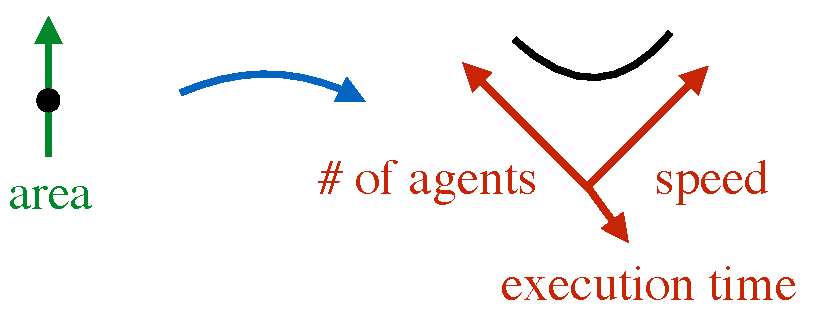
\includegraphics[scale=0.33]{reits2_multirobot2}

  }
  \caption{}
\end{figure}

\todographics{redo right-hand side in tikz}

\devel{
\subsection{LQG Control}

\todotext{Write short summary}}

\subsection{Computation}


The trivial model of a CPU is as a device that provides \Fcol{computation,
  measured in flops}, and requires \Rcol{power [W]}. Clearly there
is a monotone relation between the two.

\begin{figure}[h]
  \begin{center}
    \includesag{520_dp_cpu}
  \end{center}
  \caption{}
\end{figure}

A similar monotone relation between application requirements and computation
resources holds in a much more general setting, where both application
and computation resources are represented by graphs. This will be
an example of a monotone relation between nontrivial partial orders.

In the Static Data Flow (SDF) model of computation~\cite[Chapter 3]{sriram00,lee10},
the application is represented as a graph of procedures that need
to be allocated on a network of processors.

\begin{figure}[h]
  \begin{center}
    \subfloat[]{
      \includegraphics[scale=0.65]{reits2_small_app_graph}
    }
    \subfloat[]{
      \includegraphics[scale=0.65]{reits2_small_res_graph}
    }
    \subfloat[]{
      \includegraphics[scale=0.65]{reits2_small_allocation}
    }
  \end{center}
  \caption{}
\end{figure}


Define the\emph{ application graph }(sometimes called "computation
graph") as a graph where each node is a procedure (or "actor")
and each edge is a message that needs to be passed between procedures.
Each node is labeled by the number of ops necessary to run the procedure.
Each edge is labeled by the size of the message. There is a partial
order~$\ordleq$ on application graphs. In this order, it holds that~$A_1 \ordleq A_2$
if the application graph~$A_2$ needs more computation or bandwidth
for its execution than~$A_1$. Formally, it holds that~$A_1 \ordleq A_2$
if there is a homomorphism~$\varphi \colon A_1  \Rightarrow A_2$; and,
for each node~$n \in A_1$, the node~$\varphi(n)$ has equal or
larger computational requirements than~$n$; and for each edge~$\tup{n_1,n_2}$
in~$~A_2$, the edge~$\tup{\varphi (n_1), \varphi (n_2)}$ has equal or larger message size.


Define a \emph{resource graph} as a graph where each node represents
a processor, and each edge represents a network link. Each node is
labeled by the processor capacity [flops] Each edge is labeled
by latency [s] and bandwidth [B/s]. There is a partial order
on resources graph as well: it holds that~$R_1 \ordleq R_2$ if
the resource graph~$R_2$ has more computation or network available
than~$R_1$. The definition is similar to the case of the application
graph: there must exist a graph homomorphism~$\varphi \colon R_1  \Rightarrow R_2$
and the corresponding nodes (edges) of~$R_2$ must have larger
or equal computation (bandwidth) than those of~$R_1$.

Given an application graph~$A$ and a resource graph~$R$, a typical
resource allocation problem consists in choosing in which processor
each actor must be scheduled to maximize the throughput~$T$~[Hz].
This is equivalent to the problem of finding a graph homomorphism~$\Psi \colon A \Rightarrow R$.
Let~$T^{\ast}$ be the optimal throughput, and write it as a function
of the two graphs:
\begin{equation*}
  T^{\ast}=T^{\ast}(A,R).
\end{equation*}
Then the optimal throughput~$T^{\ast}$ is decreasing in~$A$ (a more
computationally demanding application graph decreases the throughput)
and increasing in~$R$ (more available computation/bandwidth increase
the throughput).

Therefore, we can formalize this as a design problem where the two
functionalities are \F{the throughput~$T$ [Hz]} and \F{the
application graph~$A$}, and the \R{resource graph~$R$} is the
resource.

\begin{figure}[h!]
  \begin{center}
    \includesag{dp_resourcegraph}
  \end{center}
  \caption{}
\end{figure}


\begin{example}
  Svorenova\,\,\etal~\cite{svorenova16resource} consider a joint
  sensor scheduling and control synthesis problem, in which a robot
  can decide to not perform sensing to save power, given performance
  objectives on the probability of reaching the target and the probability
  of collision. The method outputs a Pareto frontier of all possible
  operating points. This can be cast as a design problem with functionality
  equal to the \F{probability of reaching the target} and (the inverse
  of) \F{the collision probability}, and with resources equal to the
  \R{actuation power}, \R{sensing power}, and \R{sensor accuracy}.

\end{example}

\begin{figure}[h]
  \begin{center}
    \includesag{520_dp_svorenova}
  \end{center}
  \caption{\label{fig:progressive-1-1}}
\end{figure}
%\captionsideleft{\label{fig:progressive-1-1}}{\includegraphics[scale=0.33]{batteries_svorenova.pdf}}


\begin{example}
  Nardi\,\,\etal~\cite{zia16comparative} describe a benchmarking
  system for visual SLAM that provides the empirical characterization
  of the monotone relation between \F{the accuracy} of the visual
  SLAM solution, the \F{throughput {[}frames/s{]}} and \R{the energy
  for computation {[}J/frame{]}}.
  The implementation space is the product
  of algorithmic parameters, compiler flags, and architecture choices,
  such as the number of GPU cores active.
  This is an example of a design
  problem whose functionality-resources map needs to be experimentally
  evaluated.
\end{example}

\begin{figure}[h]
  \centering
  \includesag{520_dp_zia}
  \caption{}
  \label{fig:dp_zia}
\end{figure}

\subsection{Other examples in minimal robotics}

Many works have sought to find ``minimal'' designs for robots, and
can be understood as characterizing the relation between the poset
of \F{tasks} and the poset of physical resources, which is the product
of \R{sensing}, \R{actuation}, and \R{computation} resources,
plus other non-physical resources, such as \R{prior knowledge}~(\cref{fig:robot-generic}).
Given a task, there is a minimal antichain in the resources poset
that describes the possible trade-offs (for instance, compensating lousier
sensors with more computation).

\begin{figure}
  \centering
  \includegraphics[scale=0.33]{batteries_okane}
  \caption{\todo{re do in tikz}}
  \label{fig:robot-generic}
\end{figure}


\devel{
\begin{figure}
  \centering
  \includesag{dp_robotics}
  \caption{}
  \todo{finish with axes}
\end{figure}}


%\captionsideleft{\label{fig:robot-generic}}{\includegraphics[scale=0.33]{batteries_okane.pdf}}

The poset structure arises naturally: for example, in the \emph{sensor
lattice}~\cite{lavalle12sensing}, a sensor dominates another
if it induces a finer partition of the state space. Similar dominance
relations can be defined for actuation and computation. O'Kane and
Lavalle~\cite{okane08comparing} define a robot as a union of ``robotic
primitives'', where each primitive is an abstraction for a set of
sensors, actuators, and control strategies that can be used together
(for instance, a compass plus a contact sensor allow to ``drive North until
a wall is hit''). The effect of each primitive is modeled as an operator
on the robot's information space. It is possible to work out what
are the minimal combinations of robotic primitives (minimal antichain)
that are sufficient to perform a task (for instance, global localization),
and describe a dominance relation (partial order) of primitives. Other
works have focused on minimizing the complexity of the controller.
Egerstedt~\cite{egerstedt03motion} studies the relation between
the \F{complexity of the environment} and a notion of \R{minimum
description length of control strategies}, which can be taken as
a proxy for the computation necessary to perform the task. Soatto~\cite{soatto11steps}
studies the relation between the \F{performance of a visual task},
and the \R{minimal representation} that is needed to perform that
task.


\begin{example}[Hoare logic]
  \todotext{to write}
\end{example}
% !TEX root = chapter-standalone.tex


\section{Queries}
\label{sec:design-problems-querying}

A DPI is a model to which we can associate a family of optimization problems.

\todo{Connect with discussion at beginning of the part.}

One query is ``Given a lower bound on the functionality~\fun, what are the implementations that have minimal resources usage?''~(\cref{fig:setup-1}).

\begin{problem}[\FixFunMinReq]
  \label{prob:FixFunMinReq}
  \label{prob:problem1}
  Given~$\fun\in\funsp$, find the implementations in~\impsp that realize the functionality~\fun (or higher) with minimal resources, or provide a proof that there are none:
  \begin{equation}
    \begin{cases}
      \with & \imp\in\impsp,\\
      \Min_{\resleq} & \res,\\
      \subto & \res=\req(\imp),\\
      & \fun\funleq\prov(\imp).
    \end{cases}\label{eq:objective}
  \end{equation}
\end{problem}
\todo{re-do figure}
%\captionsideleft{\label{fig:setup-1}}{\includegraphics[scale=0.33]{gmcdp_setup_query_f}}

\captionsideleft{\label{fig:setup-1}}{\includesag{funresuplow_1}}


\begin{remark}[Minimal \emph{vs} least solutions]
  Note the use of~``$\Min_{\resleq}$'' in~\cref{eq:objective},
  which indicates the set of minimal (non-dominated) elements according
  to~$\resleq$, rather than~``$\min_{\resleq}$'', which would
  presume the existence of a least element. In all problems in this
  paper, the goal is to find the optimal trade-off of resources (``Pareto
  front''). So, for each~\fun, we expect to find an antichain~${\colR R}\in\Aressp$.
  We will see that this formalization allows an elegant way to treat
  multi-objective optimization. The algorithm to be developed will directly
  solve for the set~${\colR R}$, without resorting to techniques such
  as \emph{scalarization}, and therefore is able to work with arbitrary
  posets, possibly discrete.
\end{remark}


In an entirely symmetric fashion, we could fix an upper bound on
the resources usage, and then maximize the functionality provided~(\cref{fig:setup_max_f}).
The formulation is entirely dual, in the sense that it is obtained
from \cref{eq:objective} by swapping~$\Min$ with~$\Max$, \funsp~with~\ressp,
and $\prov$~with~$\req$.

\begin{problem}[\FixResMinFun]
  \label{prob:FixResMinFun}
  Given~$\res\in\ressp$, find the implementations
  in~\impsp that requires~\res (or lower)
  and provide the maximal functionality, or provide a proof that there are none:
  \begin{equation}
    \begin{cases}
      \with & \imp\in\impsp,\\
      \Max_{\funleq} & \fun,\\
      \subto & \fun=\prov(\imp),\\
      & \res\posgeq_{\ressp}\req(\imp).
    \end{cases}\label{eq:objective-1}
  \end{equation}
\end{problem}

\captionsideleft{\label{fig:setup_max_f}}{\includegraphics[scale=0.4]{gmcdp_setup_query_r}}

\vspace{1cm}
\captionsideleft{\label{fig:funresuplow_2}}{\includesag{funresuplow_2}}


Another type of query is
``Given a lower bound on the functionality~\fun
and an upper bound on the costs~\fun, what are the feasible implementations?


\begin{problem}[\FeasibleImp]
  \label{prob:FeasibleImp}
  Given~$\fun\in\funsp$ and $\res\in\ressp$, find the implementations
  in~\impsp that requires~\res (or lower)
  and provide~\fun (or higher)
  \begin{equation}
    \begin{cases}
      \with & \imp\in\impsp,\\
      \subto & \fun \funleq \prov(\imp),\\
      \subto &  \prov(\imp) \resleq \req(\imp) ,\\
    \end{cases}
  \end{equation}
\end{problem}

Another variation is to find only whether there are feasible solutions or not.

\begin{problem}[\Feasibility]
  \label{prob:Feasibility}
  Given~$\fun\in\funsp$ and $\res\in\ressp$, find if \cref{prob:FeasibleImp} is feasible.
\end{problem}

% !TEX root = chapter-standalone.tex


\section{Co-design problems}
\label{sec:Co-design-problems}


A ``co-design problem'' will be defined as a \emph{multigraph} of design
problems.
\begin{definition}[Co-design problem with implementation]
    \label{def:cdpi}
    A \emph{Co-Design Problem with Implementation} (CDPI)
    is a tuple~$\tup{\funsp,\ressp,\tup{\cdpiN,\cdpiE}}$,
    where~\funsp and~\ressp are two posets, and~$\tup{ \cdpiN,\cdpiE} $
    is a multigraph of DPIs.
    Each node~$\adp\in\cdpiN$ is a
    DPI~$\adp=\tup{\funsp_{\adp},\ressp_{\adp},\impsp_{\adp},\prov_{\adp},\req_{\adp}}.$
    An edge~$\cdpie\in\cdpiE$ is a tuple $\cdpie=\tup{ \tup{ \adp_1,\cdpiresindA} ,\tup{\adp_2,\cdpifunindB}}$,
    where~$\adp_1,\adp_2\in\cdpiN$ are two nodes and~$\cdpiresindA$
    and~$\cdpifunindB$ are the indices of the components of the functionality
    and resources to be connected, and it holds that~$\pi_{\cdpiresindA}\ressp_{\adp_1}=\pi_{\cdpifunindB}\funsp_{\adp_2}$~(\cref{fig:mcdps}).

    \begin{figure}[h]
        \centering
        \includegraphics[scale=0.33]{gmcdptro_cdpi}
        \caption{\todographicsjira{159}{redo in tikz}\label{fig:mcdps}}
    \end{figure}

\end{definition}

A CDPI is equivalent to a DPI with an implementation space~\impsp
that is a subset of the product $\prod_{\adp\in\cdpiN}\impsp_{\adp}$,
and contains only the tuples that satisfy the co-design constraints.
An implementation tuple~$\imp\in\prod_{\adp\in\cdpiN}\impsp_{\adp}$
belongs to~\impsp iff it respects all functionality--resources
constraints on the edges, in the sense that, for all edges~$\tup{\tup{ \adp_1,\cdpiresindA} ,\tup{\adp_2,\cdpifunindB}}$
in~$\cdpiE$, it holds that
\begin{equation*}
    \pi_{\cdpiresindA}\req_{\adp_1}(\pi_{\adp_1}\imp)\posleq\pi_{\cdpifunindB}\prov_{\adp_2}(\pi_{\adp_2}\imp).
\end{equation*}
The posets~$\funsp,\ressp$ for the entire CDPI are the products
of the functionality and resources of the nodes that remain \emph{unconnected}.
For a node~$\adp$, let~$\unconnectedfun_{\adp}$ and~$\unconnectedres_{\adp}$
be the set of unconnected functionalities and resources.
Then~$\funsp$ and~$\ressp$ for the CDPI are defined as the product of the unconnected functionality and resources of all DPIs:
~$\funsp=\prod_{\adp\in\cdpiN}\prod_{\cdpifunind\in\unconnectedfun_{\adp}}\pi_{\cdpifunind}\funsp_{\adp}$
and~$\ressp=\prod_{\adp\in\cdpiN}\prod_{\cdpiresind\in\unconnectedres_{\adp}}\pi_{\cdpiresind}\ressp_{\adp}.$
The maps~$\prov,\req$ return the values of the unconnected functionality
and resources:
\begin{equation*}
    \begin{aligned}
        \prov\colon \imp & \mapsto{\scriptstyle {\displaystyle \prod_{\adp\in\cdpiN}\prod_{\cdpifunind\in\unconnectedfun_{\adp}}}}\pi_{\cdpifunind}\prov_{\adp}(\pi_{\adp}\imp),\\
        \req\colon \imp & \mapsto{\displaystyle \prod_{\adp\in\cdpiN}\prod_{\cdpiresind\in\unconnectedres_{\adp}}}\pi_{\cdpiresind}\req_{\adp}(\pi_{\adp}\imp).
    \end{aligned}
\end{equation*}

\todotextjira{160}{macro for unconnected a bit similar to upper sets? }

%\devel{ % Devel because the figure is wrong.

    \begin{figure}
        \centering
        %\includegraphics[scale=0.33]{unc_atoms_g_v_graph}
        \includesag{unc_atoms_g_v_graph}
        \caption{Example of interconnection of 3 DPs}
        \label{fig:exampleq}
    \end{figure}
    \begin{example}
        The MCDP in~\cref{fig:exampleq} is the interconnection of 3
        DPs~$\adpa,\adpb,\adpc$.
        The implementation space is a subset of the product
        \begin{equation}
            \impsp_\adpa \times  \impsp_\adpb \times \impsp_\adpc.
        \end{equation}
        The elements $\tupp{\imp_\adpa, \imp_\adpb, \imp_\adpc}$ that are feasible
        are the ones that respect the following constraints:
        \begin{enumerate}
            \item Functionality and resources of each DPI are given by their implementation:
            \begin{align}
                \res_\adpa &= \req(\imp_\adpa), \\
                \res_\adpb &= \req(\imp_\adpb), \\
                \res_\adpc &= \req(\imp_\adpc), \\
                \fun_\adpa &= \prov(\imp_\adpa), \\
                \fun_\adpb &= \prov(\imp_\adpb), \\
                \fun_\adpc &= \prov(\imp_\adpc).
            \end{align}
            \item Wiring constraints:
            \begin{align}
                \tupp{\fun_{\adpa,1}, \fun_{\adpa_2}}  = \fun_\adpa, \\
                \res_{\adpb,\adpc}=\tup{\res_\adpb,\res_\adpc}, \\
                \fun_{\adpb,\adpc}=\tup{\fun_\adpb,\fun_\adpc}.
            \end{align}
            \item Co-design constraints:
            \begin{align}
                \res_{\adpb,\adpc}\posleq \fun_{\adpa,1},\\
                \res_\adpa \posleq \fun_{\adpb,\adpc}.
            \end{align}
        \end{enumerate}
    \end{example}

%}


\FloatBarrier\vfill\clearpage % keep for floats

\subsection{Recursion}

\begin{example}
    \label{exa:chassis_plus_motor}
    Consider the co-design of chassis (\cref{exa:chassis}) plus motor (\cref{exa:motor}).
    The design problem for a motor has \F{speed} and \F{torque} as the provided functionality (what the motor must provide), and \R{cost}, \R{mass}, \R{voltage}, and \R{current} as the required resources~(\cref{fig:motor}).

    \begin{figure}[h!]
        \centering
        \includesag{520_motor_dp}
        \caption{\label{fig:motor}}
    \end{figure}


    For the chassis (\cref{fig:gmcdp_chassis}), the provided functionality is parameterized by the \F{mass} of the payload and the \R{cost}, \R{total mass}, and what the chassis needs from its motor(s), such as \R{speed} and \R{torque}.

    \begin{figure}[h!]
        \centering
        \includesag{520_dp_chassis}
        \caption{\label{fig:gmcdp_chassis}}
    \end{figure}


    The two design problem can be connected at the edges for torque and speed~(\cref{fig:gmcdp_chassis_plus_motor_series}).
    The semantics is that the motor needs to have \emph{at least} the given torque and speed.

    %\begin{figure}[h]
    %  \centering
    %  \includegraphics[scale=0.33]{gmcdp_chassis_plus_motor_series}
    %  \caption{\label{fig:gmcdp_chassis_plus_motor_series}}
    %\end{figure}

    \begin{figure*}[h!]
        \centering
        \includesag{dp_chassis_motor}
        \caption{\label{fig:gmcdp_chassis_plus_motor_series}}
    \end{figure*}
%\captionsideleft{\label{fig:gmcdp_chassis_plus_motor_series}}{\includegraphics[scale=0.33]{gmcdp_chassis_plus_motor_series.pdf}}

    Resources can be summed together using a trivial DP corresponding
    to the map $\ftor:\left\langle \fun_{1},\fun_{2}\right\rangle \mapsto\{\fun_{1}+\fun_{2}\}$
    (\cref{fig:total_cost}).

    \begin{figure}
        \centering
        \includesag{520_dp_sum_costs}
        \caption{}
        \label{fig:total_cost}
    \end{figure}


%\captionsideleft{\label{fig:total_cost}}{\includegraphics[scale=0.33]{gmcdp_weightsum.pdf}}

    A co-design problem might contain recursive co-design constraints.
    For example, if we set the payload to be transported to be the sum
    of the motor mass plus some extra payload, a cycle appears in the
    graph~(\cref{fig:gmcdp_chassis_plus_motor}).


    \begin{figure}[h!]
        \centering{}
        \includegraphics[scale=0.33]{gmcdp_chassis_plus_motor}
        \caption{}
        \label{fig:gmcdp_chassis_plus_motor}
    \end{figure}

    \devel{
        \begin{center}
            \includesag{dp_chassis_motor_loop}
        \end{center}
        \todographicsjira{163}{finish dpchassismotorloop}
    }

    \FloatBarrier \vfill\clearpage

    \subsection{Abstraction}
    This formalism makes it easy to abstract away the details
    in which we are not interested. Once a diagram like~\cref{fig:gmcdp_chassis_plus_motor}
    is obtained, we can draw a box around it and consider the abstracted
    problem~(\cref{fig:gmcdp_chassis_plus_motor-1}).


    \begin{figure}[h!]
        \centering
        \includesag{520_dp_chassis_plus_motor}
        \caption{}
        \label{fig:gmcdp_chassis_plus_motor-1}
    \end{figure}

%\captionsideleft{\label{fig:gmcdp_chassis_plus_motor-1}}{\includegraphics[scale=0.33]{gmcdp_chassis_plus_motor2.pdf}}

    \label{exa:finish}Let us finish assembling our robot. A motor needs
    a motor control board. The functional requirements are the (peak)
    \F{output current} and the \F{output voltage range}~(\cref{fig:mcb}).

    \begin{figure}[h!]
        \centering
        \includesag{520_dp_board}
        \caption{}
        \label{fig:mcb}
    \end{figure}

%\captionsideleft{\label{fig:mcb}}{\includegraphics[scale=0.33]{gmcdp_mcb.pdf}}

    The functionality for a power supply could be parameterized
    by the \F{output current}, the \F{output voltages}, and the \F{capacity}.
    The resources could include \R{cost} and \R{mass} (\cref{fig:example-ba}).

    \begin{figure}[h!]
        \centering
        \includesag{520_dp_power_supply}
        \caption{\label{fig:example-ba}}
    \end{figure}


%\captionsideleft{\label{fig:example-ba}}{\includegraphics[scale=0.33]{gmcdp_battery.pdf}}

    Relations such as ${\colF\mbox{current}}\times{\colF\mbox{voltage}}\posleq{\colR\mbox{power required}}$
    and ${\colF\mbox{power}}\times{\colF\mbox{endurance}}\posleq{\colR\mbox{energy required}}$
    can be modeled by a trivial ``multiplication'' DPI (\cref{fig:current_times_voltage}).

    \begin{figure}[h!]
        \centering
        \includesag{520_dp_current_times_voltage}
        \caption{\label{fig:current_times_voltage}}
    \end{figure}

%\captionsideleft{\label{fig:current_times_voltage}}{\includegraphics[scale=0.33]{gmcdp_voltage_current.pdf}}

    We can connect these DPs to obtain a co-design problem with
    functionality \F{voltage}, \F{current}, \F{endurance} and resources
    \R{mass} and \R{cost}~(\cref{fig:connect}).

    \begin{figure}[h!]
        \centering
        \includegraphics[scale=0.29]{gmcdp_MCB_PSU_2}
        \caption{\label{fig:connect}}
    \end{figure}

%\captionsideleft{\label{fig:connect}}{\includegraphics[scale=0.29]{gmcdp_MCB_PSU_2.pdf}}

    Draw a box around the diagram, and call it ``MCB+PSU'';
    then interconnect it with the ``chassis+motor'' diagram in~\cref{fig:another}.


    \begin{figure}[h!]
        \centering
        \includegraphics[scale=0.33]{gmcdp_mobility_power}
        \caption{\label{fig:another}}
    \end{figure}

    We can further abstract away the diagram in~\cref{fig:another} as
    a ``mobility+power'' CDPI, as in \cref{fig:shipping}. The formalism
    allows to consider \R{mass} and \R{cost} as independent resources,
    meaning that we wish to obtain the Pareto frontier for the minimal
    resources. Of course, one can always reduce everything to a scalar
    objective. For example, a conversion from mass to cost exists and
    it is called ``shipping''. Depending on the destination, the conversion
    factor is between~$\$0.5/\mbox{lbs}$, using USPS, to~$\$10\mbox{k}/\mbox{lbs}$
    for sending your robot to low Earth orbit.


    \begin{figure}[h!]
        \centering{}
        \includegraphics[scale=0.33]{gmcdp_shipping}\caption{\label{fig:shipping}}
    \end{figure}

\end{example}


% !TEX root = chapter-standalone.tex

\section{Discussion of related work}
\label{sec:design-problems-related}

\subsection{Theory of design}

Modern engineering has long since recognized the two ideas of modularity and hierarchical decomposition, yet there exists no general quantitative theory of design that is applicable to different domains.
Most of the works in the theory of design literature study abstractions that are meant to be useful for a human designer, rather than an automated system.
For example, a \emph{function structure} diagram~\cite[p.
    32]{pahl07} decomposes the function of a system in subsystems that exchange energy,
materials, and signals, but it is not a formal representation.
From the point of view of the theory of design, the contribution of this work is that the \emph{design problem} abstraction developed, where one takes functionality and resources as the interfaces for the subsystems, is at the same time (1) mathematically precise; (2)~intuitive to understand; and (3)~leads to tractable optimization problems.

This work also provides a clear answer to one long-standing issue in the theory of design: the inter-dependence between subsystems, (in other words, cycles in the co-design graph).
Consider, as an example, Suh's theory of \emph{axiomatic design~}\cite{suh01}, in which the first ``axiom'' is to keep the design requirements orthogonal (in other words, do not introduce cycles).
This work shows that it is possible to deal elegantly with recursive constraints.

\subsection{Partial Order Programming}

In ``Partial Order Programming''~\cite{parkerjr89partial} Parker studies a hierarchy of optimization problems that can be represented as a set of partial order constraints.
The main interest is to study partial order constraints as the means to define the semantics of programming languages and for declarative approaches to knowledge representation.

In Parker's hierarchy, CDPIs are most related to the class of problems called \emph{continuous monotone partial order program} (CMPOP).
CMPOPs are the least specific class of problems studied by Parker for which it is possible to obtain existence results and a systematic solution procedure.
CDPIs subsume CMPOPs.
A CMPOP is an CDPIs where: 1)~All functionality and resources belong to the same poset~\posA ($\funsp_{v}=\ressp_{v}=\posA$);
2)~Each functionality/resource relation is a simple map, rather than a multivalued relation; 3)~There are no dangling functionality edges in the co-design diagram ($\funsp=\One$).

In a CDPI, each DP is described by a \SY{Scott continuous} map~$\ftor:\funsp\rightarrow\Aressp$ which maps one functionality to a minimal set of resources.
By contrast, in a CMPOP an operator corresponds to a \SY{Scott continuous} map~$\ftor:\funsp\rightarrow\ressp$.
The consequence is that a CMPOP has a unique solution~\cite[Theorem 8]{parkerjr89partial},
while an CDPI can have multiple minimal solutions (or none at all).
\todotext{@AC: note here we use the other notation with \SY{antichains} }

\subsection{Abstract interpretation}

The methods used from order theory are the same used in the field of \emph{abstract interpretation}~\cite{cousot14abstract}.
In that field, the \SY{least fixed point} semantics arises from problems such as computing the sets of reachable states.
Given a starting state,
one is interested to find a subset of states that is closed under the dynamics (in other words, a fixed point), and that is the smallest that contains the given initial state (in other words, a \emph{least} fixed point).
Reachability and other properties lead to considering systems of equation of the form
\begin{align}
    x_{i} & =\varphi_{i}(x_{1},\,\dots\,,x_{i},\,\dots\,,x_{n}),\quad i=1,\dots,n,\label{eq:ai}
\end{align}
where each value of the index $i$ is for a control point of the program, and~$\varphi_{i}$ are \SY{Scott continuous} functions on the abstract \SY{lattice} that represents the properties of the program.
In the simplest case, each~$x_{i}$ could represent intervals that a variable could assume at step~$i$.
By applying the iterations, one finds which properties can be inferred to be valid at each step.

We can repeat the same considerations we did for Parker's CMPOPs \vs CDPIs.
In particular, in a CDP we deal with multivalued maps, and there is more than one solution.

In the field of abstract interpretation much work has been done towards optimizing the rate of convergence.
The order of evaluation in~\cref{eq:ai} does not matter.
Asynchronous and ``chaotic'' iterations were proposed early~\cite{cousot77asynchronous} and are still object of investigation~\cite{bourdoncleefficient}.
To speed up convergence, the so-called ``widening'' and ``narrowing'' operators are used~\cite{cortesi11widening}.
The ideas of chaotic iteration, widening, narrowing, are not immediately applicable to CDPs, but it is a promising research direction.


